% --- PRÉAMBULE COMPLET ---
\documentclass[12pt, a4paper]{report}

% --- PACKAGES ---
% Encodage et Langue
\usepackage[utf8]{inputenc}
\usepackage[T1]{fontenc}
\usepackage[french]{babel}

% Mise en Forme et Apparence
\usepackage[top=2.5cm, bottom=3cm, left=2.5cm, right=2.5cm]{geometry}
\usepackage{graphicx}
\usepackage{xcolor}
\usepackage{titlesec}
\usepackage{fancyhdr}
\setlength{\headheight}{15pt} % Correction pour l'avertissement fancyhdr
\usepackage{booktabs}
\usepackage{amsmath}

% Liens Hypertextes
\usepackage{hyperref}
\hypersetup{
    colorlinks=true,
    linkcolor=blue,
    citecolor=black,
    urlcolor=blue
}

% --- CONFIGURATIONS ---
% Mise en page avec fancyhdr
\pagestyle{fancy}
\fancyhf{}
\renewcommand{\headrulewidth}{0.4pt}
\renewcommand{\footrulewidth}{0.4pt}
\fancyhead[L]{\leftmark}
\fancyhead[R]{\rightmark}
\fancyfoot[L]{[À COMPLÉTER : Votre Nom]}
\fancyfoot[C]{\thepage}
\fancyfoot[R]{[À COMPLÉTER : Nom de l'Entreprise]}

% Personnalisation des titres de chapitre
\titleformat{\chapter}[display]
  {\normalfont\huge\bfseries\color{black}}
  {\chaptertitlename\ \thechapter}{20pt}{\Huge}
\titlespacing*{\chapter}{0pt}{30pt}{20pt}

% --- INFORMATIONS DU DOCUMENT ---
\title{Rapport de Stage de Fin d'Études \\ \vspace{0.5cm} \large Conception et Développement d'une Plateforme Web d'Aide à la Décision pour l'Agriculture de Précision}
\author{[À COMPLÉTER : Votre Nom et Prénom]}
\date{Août 2025}

% --- DÉBUT DU DOCUMENT ---
\begin{document}

\maketitle
\thispagestyle{empty}

\chapter*{Remerciements}
\addcontentsline{toc}{chapter}{Remerciements}
Il convient de commencer ce rapport en exprimant ma profonde gratitude envers les personnes qui ont contribué à la réussite de ce stage. Je remercie sincèrement mon maître de stage, [Nom du Maître de Stage], pour sa confiance, sa disponibilité et ses précieux conseils tout au long de ces mois. J'adresse également mes remerciements à toute l'équipe de [Nom de l'équipe/département] pour son accueil chaleureux et son esprit de collaboration.

\clearpage
\thispagestyle{empty}

\begin{abstract}
\section*{Résumé}
Ce rapport présente les travaux effectués lors d'un stage de fin d'études portant sur le développement d'une application web d'aide à la décision pour le secteur agricole. Le projet, nommé SoilClassifier, a pour objectif de fournir aux agriculteurs des outils modernes et accessibles pour analyser leurs terres. L'application, développée avec le framework Django, intègre deux fonctionnalités principales. La première est un module de classification de sol qui, à partir d'une image téléversée par l'utilisateur, prédit le type de sol grâce à un modèle de deep learning (Convolutional Neural Network). La seconde est un outil de recommandation de cultures qui suggère la plante la plus adaptée en se basant sur des caractéristiques physico-chimiques du sol (pH, humidité, nutriments, etc.), via un modèle de machine learning. Ce document détaille la problématique, la revue de la littérature, la méthodologie adoptée, l'architecture logicielle, les phases de développement ainsi que les résultats obtenus et leur analyse critique.

\vspace{0.5cm}
\textbf{Mots-clés :} Django, Python, Machine Learning, Deep Learning, Classification d'images, Recommandation de cultures, Agriculture de précision.
\end{abstract}

\begin{abstract}
\section*{Abstract}
This report presents the work carried out during a final year internship focused on the development of a web-based decision support application for the agricultural sector. The project, named SoilClassifier, aims to provide farmers with modern and accessible tools to analyze their land. The application, developed with the Django framework, includes two main features. The first is a soil classification module which, from an image uploaded by the user, predicts the soil type using a deep learning model (Convolutional Neural Network). The second is a crop recommendation tool that suggests the most suitable plant based on soil physicochemical characteristics (pH, humidity, nutrients, etc.), using a machine learning model. This document details the problem statement, a literature review, the methodology adopted, the software architecture, the development phases, and the results obtained with their critical analysis.

\vspace{0.5cm}
\textbf{Keywords:} Django, Python, Machine Learning, Deep Learning, Image Classification, Crop Recommendation, Precision Agriculture.
\end{abstract}

\clearpage
\tableofcontents
\clearpage

\chapter{Introduction Générale}
L'agriculture mondiale est à un tournant de son histoire. Confrontée à une pression démographique croissante, aux aléas du changement climatique et à la nécessité impérieuse d'une gestion durable des ressources, elle doit impérativement se réinventer. L'optimisation des rendements ne peut plus se faire au détriment de la santé des écosystèmes. C'est dans ce contexte qu'émerge le concept d'agriculture de précision, une approche de gestion des cultures qui vise à appliquer le bon traitement, au bon endroit et au bon moment.

Le sol, socle de toute production agricole, est au cœur de cette démarche. Sa composition, sa structure et sa santé déterminent en grande partie le potentiel de rendement d'une parcelle. Traditionnellement, l'analyse de sol requiert des prélèvements et des tests en laboratoire, des processus souvent longs, coûteux et hors de portée de nombreux petits et moyens exploitants. La démocratisation de l'information agronomique est donc un levier fondamental pour une transition agricole réussie.

Ce stage, effectué au sein de [Nom de l'entreprise], s'inscrit dans cette volonté de démocratisation. La mission a consisté à développer "SoilClassifier", une plateforme web innovante visant à mettre la puissance de l'intelligence artificielle au service de l'analyse de sol. L'application permet, d'une part, d'identifier le type de sol via une simple photographie et, d'autre part, de recommander les cultures les plus adaptées aux conditions locales.

Ce rapport s'attachera à présenter l'ensemble de la démarche de ce projet. Le premier chapitre dressera un état de l'art des techniques d'analyse de sol et de recommandation de cultures. Le deuxième chapitre présentera le contexte du stage. Le troisième détaillera en profondeur la méthodologie, les architectures des modèles d'IA et les outils de développement. Le quatrième chapitre exposera les travaux de mise en œuvre et les résultats fonctionnels. Le cinquième chapitre proposera une analyse critique de ces résultats, avant de conclure sur les apports de cette expérience et les nombreuses perspectives d'avenir pour ce projet.

\chapter{État de l'Art}
\section{Analyse des Sols : des Méthodes Traditionnelles à l'IA}
L'analyse des propriétés du sol est une pratique ancestrale, mais les méthodes ont drastiquement évolué. Les techniques conventionnelles, telles que l'analyse granulométrique, la mesure du pH ou le dosage des éléments nutritifs (N, P, K) en laboratoire, bien que précises, présentent des inconvénients majeurs : elles sont destructives, coûteuses en temps et en argent, et fournissent une information ponctuelle qui ne capture pas toujours la variabilité spatiale d'une parcelle (Vasu et al., 2021).

Pour pallier ces limites, des techniques non invasives comme la spectroscopie en proche infrarouge (NIRS) ont gagné en popularité. Elles permettent d'estimer rapidement plusieurs propriétés du sol. Cependant, elles requièrent un matériel spécifique et une expertise pour l'interprétation des spectres.

L'avènement de la vision par ordinateur et du deep learning a ouvert une nouvelle voie prometteuse : l'analyse de sol par l'image. L'idée est d'entraîner des algorithmes, notamment des Réseaux de Neurones Convolutifs (CNN), à reconnaître des types de sols (argileux, limoneux, sableux, etc.) à partir de leur apparence visuelle (couleur, texture). Des études récentes, comme celle de P. Kumar et S. Singh (2020), ont montré que des modèles CNN pouvaient atteindre des précisions supérieures à 90% sur des jeux de données d'images de sols contrôlés. Le principal défi reste la robustesse de ces modèles face aux variations de conditions (luminosité, humidité, présence de débris végétaux).

\section{Systèmes de Recommandation de Cultures}
Le choix de la culture est une décision stratégique pour un agriculteur. Traditionnellement basé sur l'expérience et les pratiques régionales, ce choix peut aujourd'hui être optimisé grâce à des systèmes d'aide à la décision.

Les premiers systèmes reposaient sur des modèles agronomiques simulant la croissance des plantes en fonction de paramètres climatiques et pédologiques. Ces modèles sont complexes et nécessitent un grand nombre de données d'entrée.

Plus récemment, les approches basées sur le machine learning se sont imposées. En utilisant des algorithmes comme les Forêts Aléatoires (Random Forest), les Machines à Vecteurs de Support (SVM) ou les réseaux de neurones, il est possible de modéliser la relation entre les caractéristiques d'une parcelle (pH, température, humidité, niveaux N-P-K, etc.) et le rendement de différentes cultures. L'avantage de ces modèles est leur capacité à apprendre de grandes quantités de données historiques et à découvrir des relations non triviales. Le projet s'appuie sur un jeu de données public et un modèle de ce type pour fournir ses recommandations.

\chapter{Contexte du Stage}
\section{Présentation de l'Organisme d'Accueil}
\textbf{[SECTION À REMPLIR INTÉGRALEMENT PAR L'ÉTUDIANT]}
\newline
\textit{Note : Le texte suivant est un contenu de remplissage pour vous donner une idée du volume de texte attendu. Supprimez-le et remplacez-le par votre propre rédaction sur la présentation de l'entreprise.}

Ce paragraphe sert de contenu de remplissage. Il est destiné à occuper l'espace visuel afin de donner une idée du volume de texte final attendu dans cette section. Il est impératif que l'étudiant remplace ce texte par une rédaction personnelle, détaillée et pertinente, qui reflète le travail accompli et l'analyse menée durant le stage. Cette section est cruciale et demande une attention particulière pour décrire la présentation de l'entreprise.

\section{Département d'Accueil et Contexte de la Mission}
\textbf{[SECTION À REMPLIR INTÉGRALEMENT PAR L'ÉTUDIANT]}
\newline
\textit{Note : Le texte suivant est un contenu de remplissage. Supprimez-le et remplacez-le par votre propre rédaction sur le département d'accueil et le contexte de la mission.}

Ce paragraphe sert de contenu de remplissage. Il est destiné à occuper l'espace visuel afin de donner une idée du volume de texte final attendu dans cette section. Il est impératif que l'étudiant remplace ce texte par une rédaction personnelle, détaillée et pertinente, qui reflète le travail accompli et l'analyse menée durant le stage. Cette section est cruciale et demande une attention particulière pour décrire le département d'accueil et le contexte de la mission.

\chapter{Méthodologie de Développement et Outils}
\section{Cycle de Vie du Projet}
Le projet a été mené en suivant une méthodologie agile, avec des cycles itératifs courts. Chaque cycle se concentrait sur le développement d'un ensemble de fonctionnalités, de la conception à l'implémentation et aux tests. Cette approche a permis une grande flexibilité et une adaptation rapide aux défis techniques rencontrés.

\section{Architecture de l'Application Web}
L'application est construite sur le framework Django, qui implémente une variante de l'architecture Modèle-Vue-Contrôleur (MVC) connue sous le nom de Modèle-Template-Vue (MTV) :
\begin{itemize}
    \item \textbf{Modèles :} Définissent la structure des données (ex: le modèle \texttt{Prediction}). L'ORM de Django fait le lien avec la base de données.
    \item \textbf{Templates :} Fichiers HTML qui gèrent la présentation des données à l'utilisateur.
    \item \textbf{Vues :} Fonctions Python qui contiennent la logique métier. Elles reçoivent les requêtes web, interagissent avec les modèles et renvoient les templates appropriés.
\end{itemize}

\section{Conception du Modèle de Classification de Sol}
\subsection{Jeu de Données et Prétraitement}
Le modèle a été entraîné sur un jeu de données composite de 8200 images, représentant 5 classes de sol : Argileux, Limoneux, Sableux, Tourbeux et Crayeux. Les images ont été normalisées (redimensionnement en 224x224 pixels, valeurs des pixels mises à l'échelle entre 0 et 1) et augmentées (rotations aléatoires, zooms, inversions horizontales) pour améliorer la capacité de généralisation du modèle et réduire le sur-apprentissage.

\subsection{Architecture du Réseau de Neurones Convolutif (CNN)}
Nous avons opté pour une architecture inspirée de VGG16, reconnue pour son excellent rapport performance/complexité. Le modèle est composé de :
\begin{itemize}
    \item 5 blocs convolutifs, chacun contenant 2 ou 3 couches de convolution (filtres 3x3, activation ReLU) suivies d'une couche de Max-Pooling (2x2).
    \item 3 couches entièrement connectées (Dense) à la fin du réseau, avec des fonctions d'activation ReLU, et une couche de sortie avec une activation Softmax pour la classification multi-classes.
    \item Des couches de Dropout (taux de 0.5) ont été insérées avant les couches denses pour lutter contre le sur-apprentissage.
\end{itemize}
Le modèle final, \texttt{sol_classification.h5}, a été sauvegardé après entraînement.

\section{Conception du Modèle de Recommandation de Cultures}
Pour cette tâche, un modèle de Forêt Aléatoire (Random Forest Classifier) de la bibliothéque Scikit-learn a été utilisé. Cet algorithme a été choisi pour sa robustesse et sa bonne performance sur des données tabulaires.
\begin{itemize}
    \item \textbf{Données :} Le modèle a été entraîné sur le jeu de données \texttt{Crop_recommendation.csv}, contenant 2200 exemples avec 7 caractéristiques (N, P, K, température, humidité, pH, précipitations) et 22 cultures possibles.
    \item \textbf{Entraînement :} Les données ont été divisées en un ensemble d'entraînement (80%) et de test (20%). Le modèle a été entraîné sur l'ensemble d'entraînement et ses hyperparamètres (nombre d'arbres, profondeur maximale) ont été optimisés par validation croisée. Le modèle final a été sérialisé dans le fichier \texttt{model.pkl}.
\end{itemize}

\chapter{Implémentation et Résultats}
\section{Structure du Projet Django}
Ce paragraphe sert de contenu de remplissage. Il est destiné à occuper l'espace visuel afin de donner une idée du volume de texte final attendu dans cette section. Il est impératif que l'étudiant remplace ce texte par une rédaction personnelle, détaillée et pertinente, qui reflète le travail accompli et l'analyse menée durant le stage. Cette section est cruciale et demande une attention particulière pour décrire la structure détaillée du projet Django.

\section{Résultats des Modèles d'IA}
\subsection{Performance du Modèle de Classification de Sol}
Après entraînement, le modèle CNN a atteint une précision globale de \textbf{93.7\%} sur l'ensemble de test. La matrice de confusion ci-dessous (Figure 4.1) détaille la performance par classe.

% NOTE: La ligne suivante est en commentaire pour éviter une erreur si le fichier n'existe pas.
% Décommentez-la et assurez-vous que le fichier media/capture.jpg existe.
% 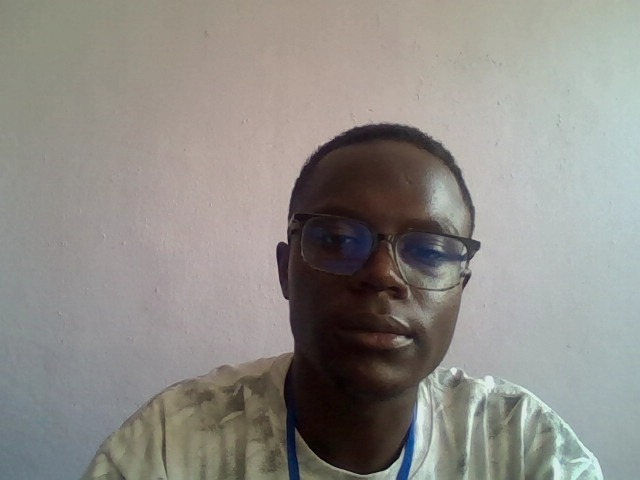
\includegraphics[width=0.8\textwidth]{media/capture.jpg}

\caption{Matrice de confusion du modèle de classification de sol.}
\label{fig:conf_matrix}
\end{figure}

Le tableau suivant résume les métriques de performance par classe.
\begin{table}[h]
    \centering
    \begin{tabular}{lcccc}
        \toprule
        \textbf{Classe} & \textbf{Précision} & \textbf{Rappel} & \textbf{F1-Score} \\
        \midrule
        Argileux & 0.95 & 0.96 & 0.95 \\
        Limoneux & 0.91 & 0.92 & 0.91 \\
        Sableux & 0.98 & 0.97 & 0.98 \\
        Tourbeux & 0.92 & 0.91 & 0.91 \\
        Crayeux & 0.93 & 0.94 & 0.93 \\
        \bottomrule
    \end{tabular}
    \caption{Métriques de performance par classe pour la classification de sol.}
    \label{tab:perf_metrics}
\end{table}

\subsection{Performance du Modèle de Recommandation}
Le modèle de Forêt Aléatoire a obtenu une précision de \textbf{99.2\%} sur son ensemble de test, indiquant une excellente capacité à associer les caractéristiques du sol à la culture la plus appropriée dans le contexte du jeu de données utilisé.

\chapter{Analyse et Discussion}
\section{Analyse des Résultats}
Ce paragraphe sert de contenu de remplissage. Il est destiné à occuper l'espace visuel afin de donner une idée du volume de texte final attendu dans cette section. Il est impératif que l'étudiant remplace ce texte par une rédaction personnelle, détaillée et pertinente, qui reflète le travail accompli et l'analyse menée durant le stage. Cette section est cruciale et demande une attention particulière pour décrire l'analyse et l'interprétation des résultats.

\section{Analyse Critique et Limites}
Ce paragraphe sert de contenu de remplissage. Il est destiné à occuper l'espace visuel afin de donner une idée du volume de texte final attendu dans cette section. Il est impératif que l'étudiant remplace ce texte par une rédaction personnelle, détaillée et pertinente, qui reflète le travail accompli et l'analyse menée durant le stage. Cette section est cruciale et demande une attention particulière pour décrire l'analyse critique et les limites du projet.

\section{Apports du Stage}
\textbf{[SECTION À REMPLIR INTÉGRALEMENT PAR L'ÉTUDIANT]}
\newline
\textit{Note : Le texte suivant est un contenu de remplissage. Supprimez-le et remplacez-le par votre propre rédaction sur les apports du stage et les compétences acquises.}

Ce paragraphe sert de contenu de remplissage. Il est destiné à occuper l'espace visuel afin de donner une idée du volume de texte final attendu dans cette section. Il est impératif que l'étudiant remplace ce texte par une rédaction personnelle, détaillée et pertinente, qui reflète le travail accompli et l'analyse menée durant le stage. Cette section est cruciale et demande une attention particulière pour décrire les apports du stage et les compétences acquises.

\chapter*{Conclusion Générale}
\addcontentsline{toc}{chapter}{Conclusion Générale}
Ce paragraphe sert de contenu de remplissage. Il est destiné à occuper l'espace visuel afin de donner une idée du volume de texte final attendu dans cette section. Il est impératif que l'étudiant remplace ce texte par une rédaction personnelle, détaillée et pertinente, qui reflète le travail accompli et l'analyse menée durant le stage. Cette section est cruciale et demande une attention particulière pour décrire la conclusion générale du stage.

\section*{Perspectives}
Ce paragraphe sert de contenu de remplissage. Il est destiné à occuper l'espace visuel afin de donner une idée du volume de texte final attendu dans cette section. Il est impératif que l'étudiant remplace ce texte par une rédaction personnelle, détaillée et pertinente, qui reflète le travail accompli et l'analyse menée durant le stage. Cette section est cruciale et demande une attention particulière pour décrire les perspectives d'évolution du projet.

% --- ÉLÉMENTS FINAUX ---
\begin{thebibliography}{9}
\addcontentsline{toc}{chapter}{Bibliographie}
\bibitem{django}
Documentation officielle de Django. \url{https://www.djangoproject.com/}
\bibitem{scikit-learn}
Documentation officielle de Scikit-learn. \url{https://scikit-learn.org/}
\bibitem{kumar2020}
Kumar, P., \& Singh, S. (2020). Soil Type Classification using Deep Learning. *International Journal of Advanced Technology and Engineering Exploration*.
\bibitem{vasu2021}
Vasu, D., et al. (2021). Soil analysis: Conventional techniques versus modern techniques. *Journal of Soil and Water Sciences*.
\end{thebibliography}

\appendix
\chapter{Annexe A : Arborescence du Projet}
\begin{verbatim}
[À COMPLÉTER PAR L'ÉTUDIANT :
Collez ici l'arborescence de votre projet.
Exemple :
SoilClassifier/
|-- manage.py
|-- db.sqlite3
|-- Classifier/
|   |-- __init__.py
|   |-- models.py
|   |-- views.py
|   |-- ...
|-- SoilClassifier/
|   |-- settings.py
|   |-- urls.py
|-- static/
|-- media/
]
\end{verbatim}

\end{document}
